\chapter{QASM: Question and Answer Social Media}
\doublespacing
\label{chap:qasm}
\minitoc

\section{Introduction: formalizing and linking knowledge on Q\&A sites}
Community Question Answering (CQA) services provide a platform where users can ask expert for help. Since questions and answers can be viewed and discussed and that all these traces can be searched afterwards, QA sites form a special kind of social media.

% TODO: avoid repeating sentences as the following one and try to have introductions specific to the chaper (I modified the text above for that) "people with similar questions can also directly find solutions by browsing this content. Therefore, effectively managing these content is a key issue." 

In order to make the data of a social media available on the semantic Web we have to perform two steps:

\begin{itemize}
\item \textbf{extracting and formalizing:} to choose or provide suitable vocabularies or extensions to represent the social media data (content, users, interactions, etc.) and provide the extraction mechanism to produce the semantic Web representation from the native structures and APIs of the social media platform. This is what we address in this chapter.
\item \textbf{linking:} to weave a Web of data and allow the extracted data to be fully linked to other sources of the Web of data benefiting from this enrichment and contributing to the creation of new pathways in the linked data. This will be covered in Chapter \ref{chap:label}
\end{itemize}

We also differentiate between two kinds of information in our scenario.
\begin{itemize}
\item \textbf{Information explicitly generated:} this is the original user-generated content, for instance, a question, an answer, a comment, a tag etc.
\item \textbf{Information implicitly generated:}  this information is generated as a side effect of the activity on the site. This is latent information extracted by data mining techniques, for instance, implicit social networks, detected community, traces and logs temporal information etc.
\end{itemize}



It is important to formalize both kinds of information and to link the obtained representations in order to benefit from both aspects in the analysis. Among the available vocabularies (e.g. in the LOV directory) the SIOC\footnote{\url{http://lov.okfn.org/dataset/lov/vocabs/sioc} (accessed Aug 2016)} ontology is the most popular vocabulary to formalize social medias, but it does not support the formalization of the latent information extracted by data mining techniques.


In this chapter, we propose the QASM (Question \& Answer Social Media) vocabulary. We reuse existing vocabularies such as SIOC and FOAF\footnote{\url{http://lov.okfn.org/dataset/lov/vocabs/foaf} (accessed Aug 2016)} and extend them with the primitives needed to formalize explicit and implicit QA social media.


\section{Overview of our modeling approach}
Figure \ref{fig:overview} presents an overview of QASM. We first use the SIOC ontology\footnote{\url{http://sioc-project.org/ontology} (accessed Aug 2016)} to construct an RDF dataset from social media data extracted from a CQA site, namely StackOverflow. Then we use social media mining techniques to extract topics, interests and expertise levels and temporal dyanmics from this dataset. We formalize them with the QASM vocabulary and enrich our RDF dataset with these latent information. As a result, we provide an integrated and enriched Q\&A triple store which contains both user interests, user expertise, and temporal dynamics of users'profiles and of topics. 
Then, we link our dataset with DBpedia and use the resulting knowledge graph to generate labels for topics. Finally, based on the QASM RDF dataset, we can provide the users of the Q\&A site with several services to find relevant experts for a question and to search for similar questions.

\begin{figure}%[htbp]
\centering
%\epsfig{file=fly.eps, height=1in, width=1in} % use this if you use "pdflatex"
%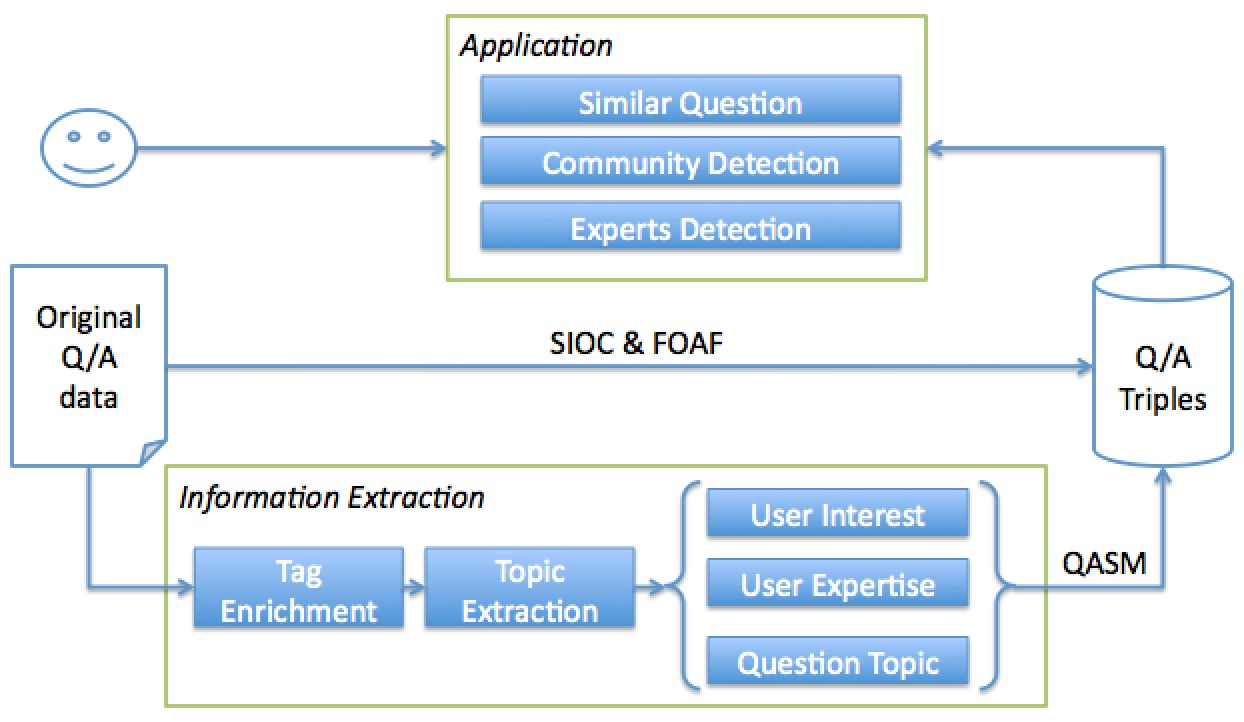
\includegraphics[height=1.857in, width=3.2in]{overview.png}  
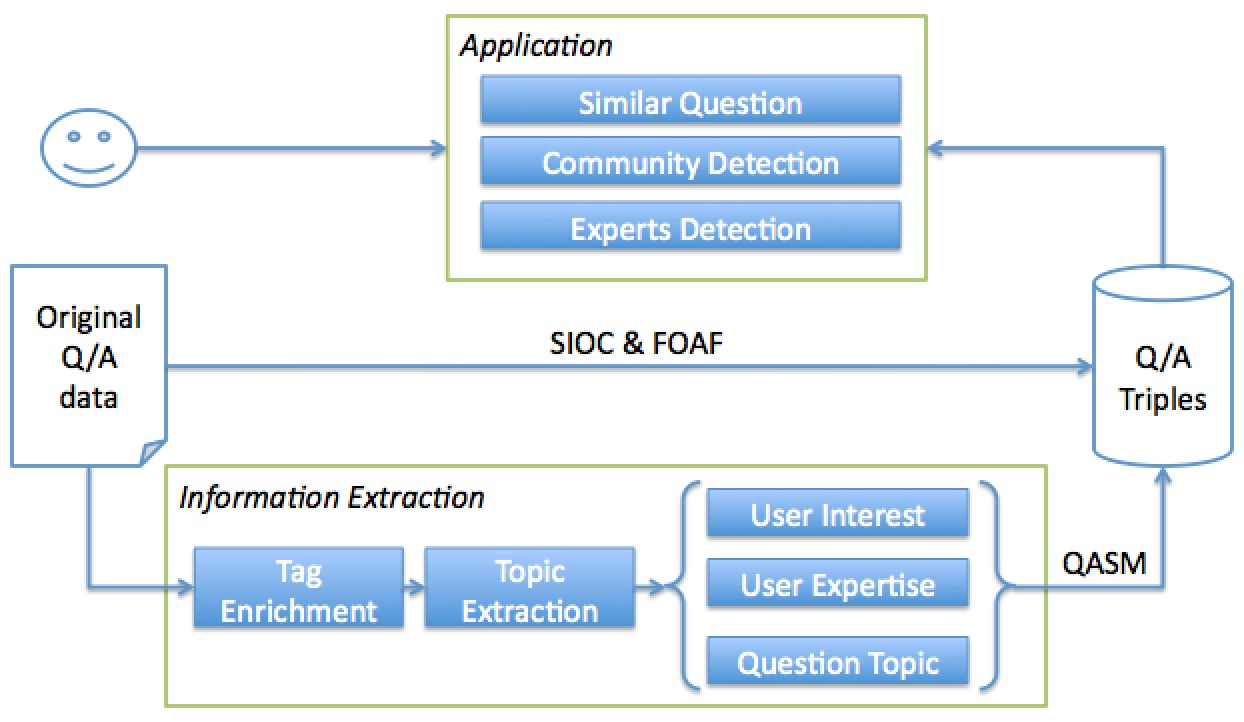
\includegraphics[width=5in]{overview.png}  
\caption{Overview of QASM}
\label{fig:overview} 
\end{figure}

\section{QASM Vocabulary: formalize Q\&A information}
%\begin{figure}[htbp]
\begin{sidewaysfigure}
\centering
%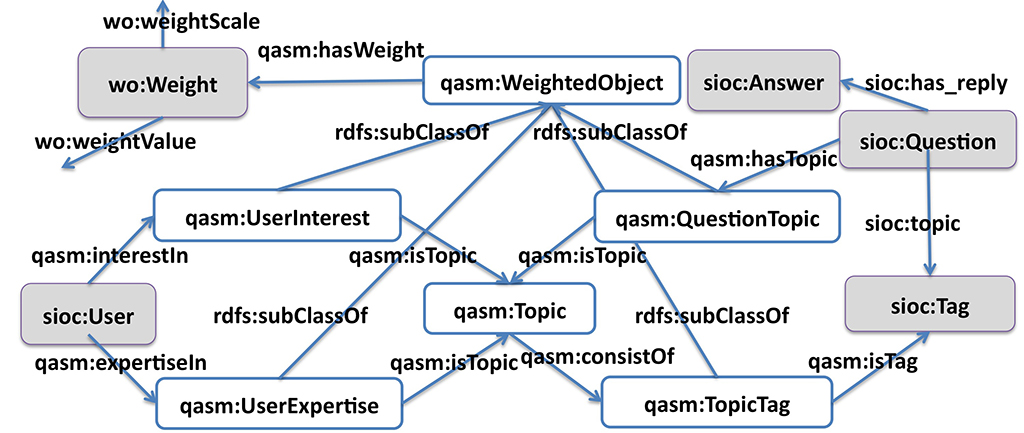
\includegraphics[width=3.7in]{ontologyv2.jpg}  
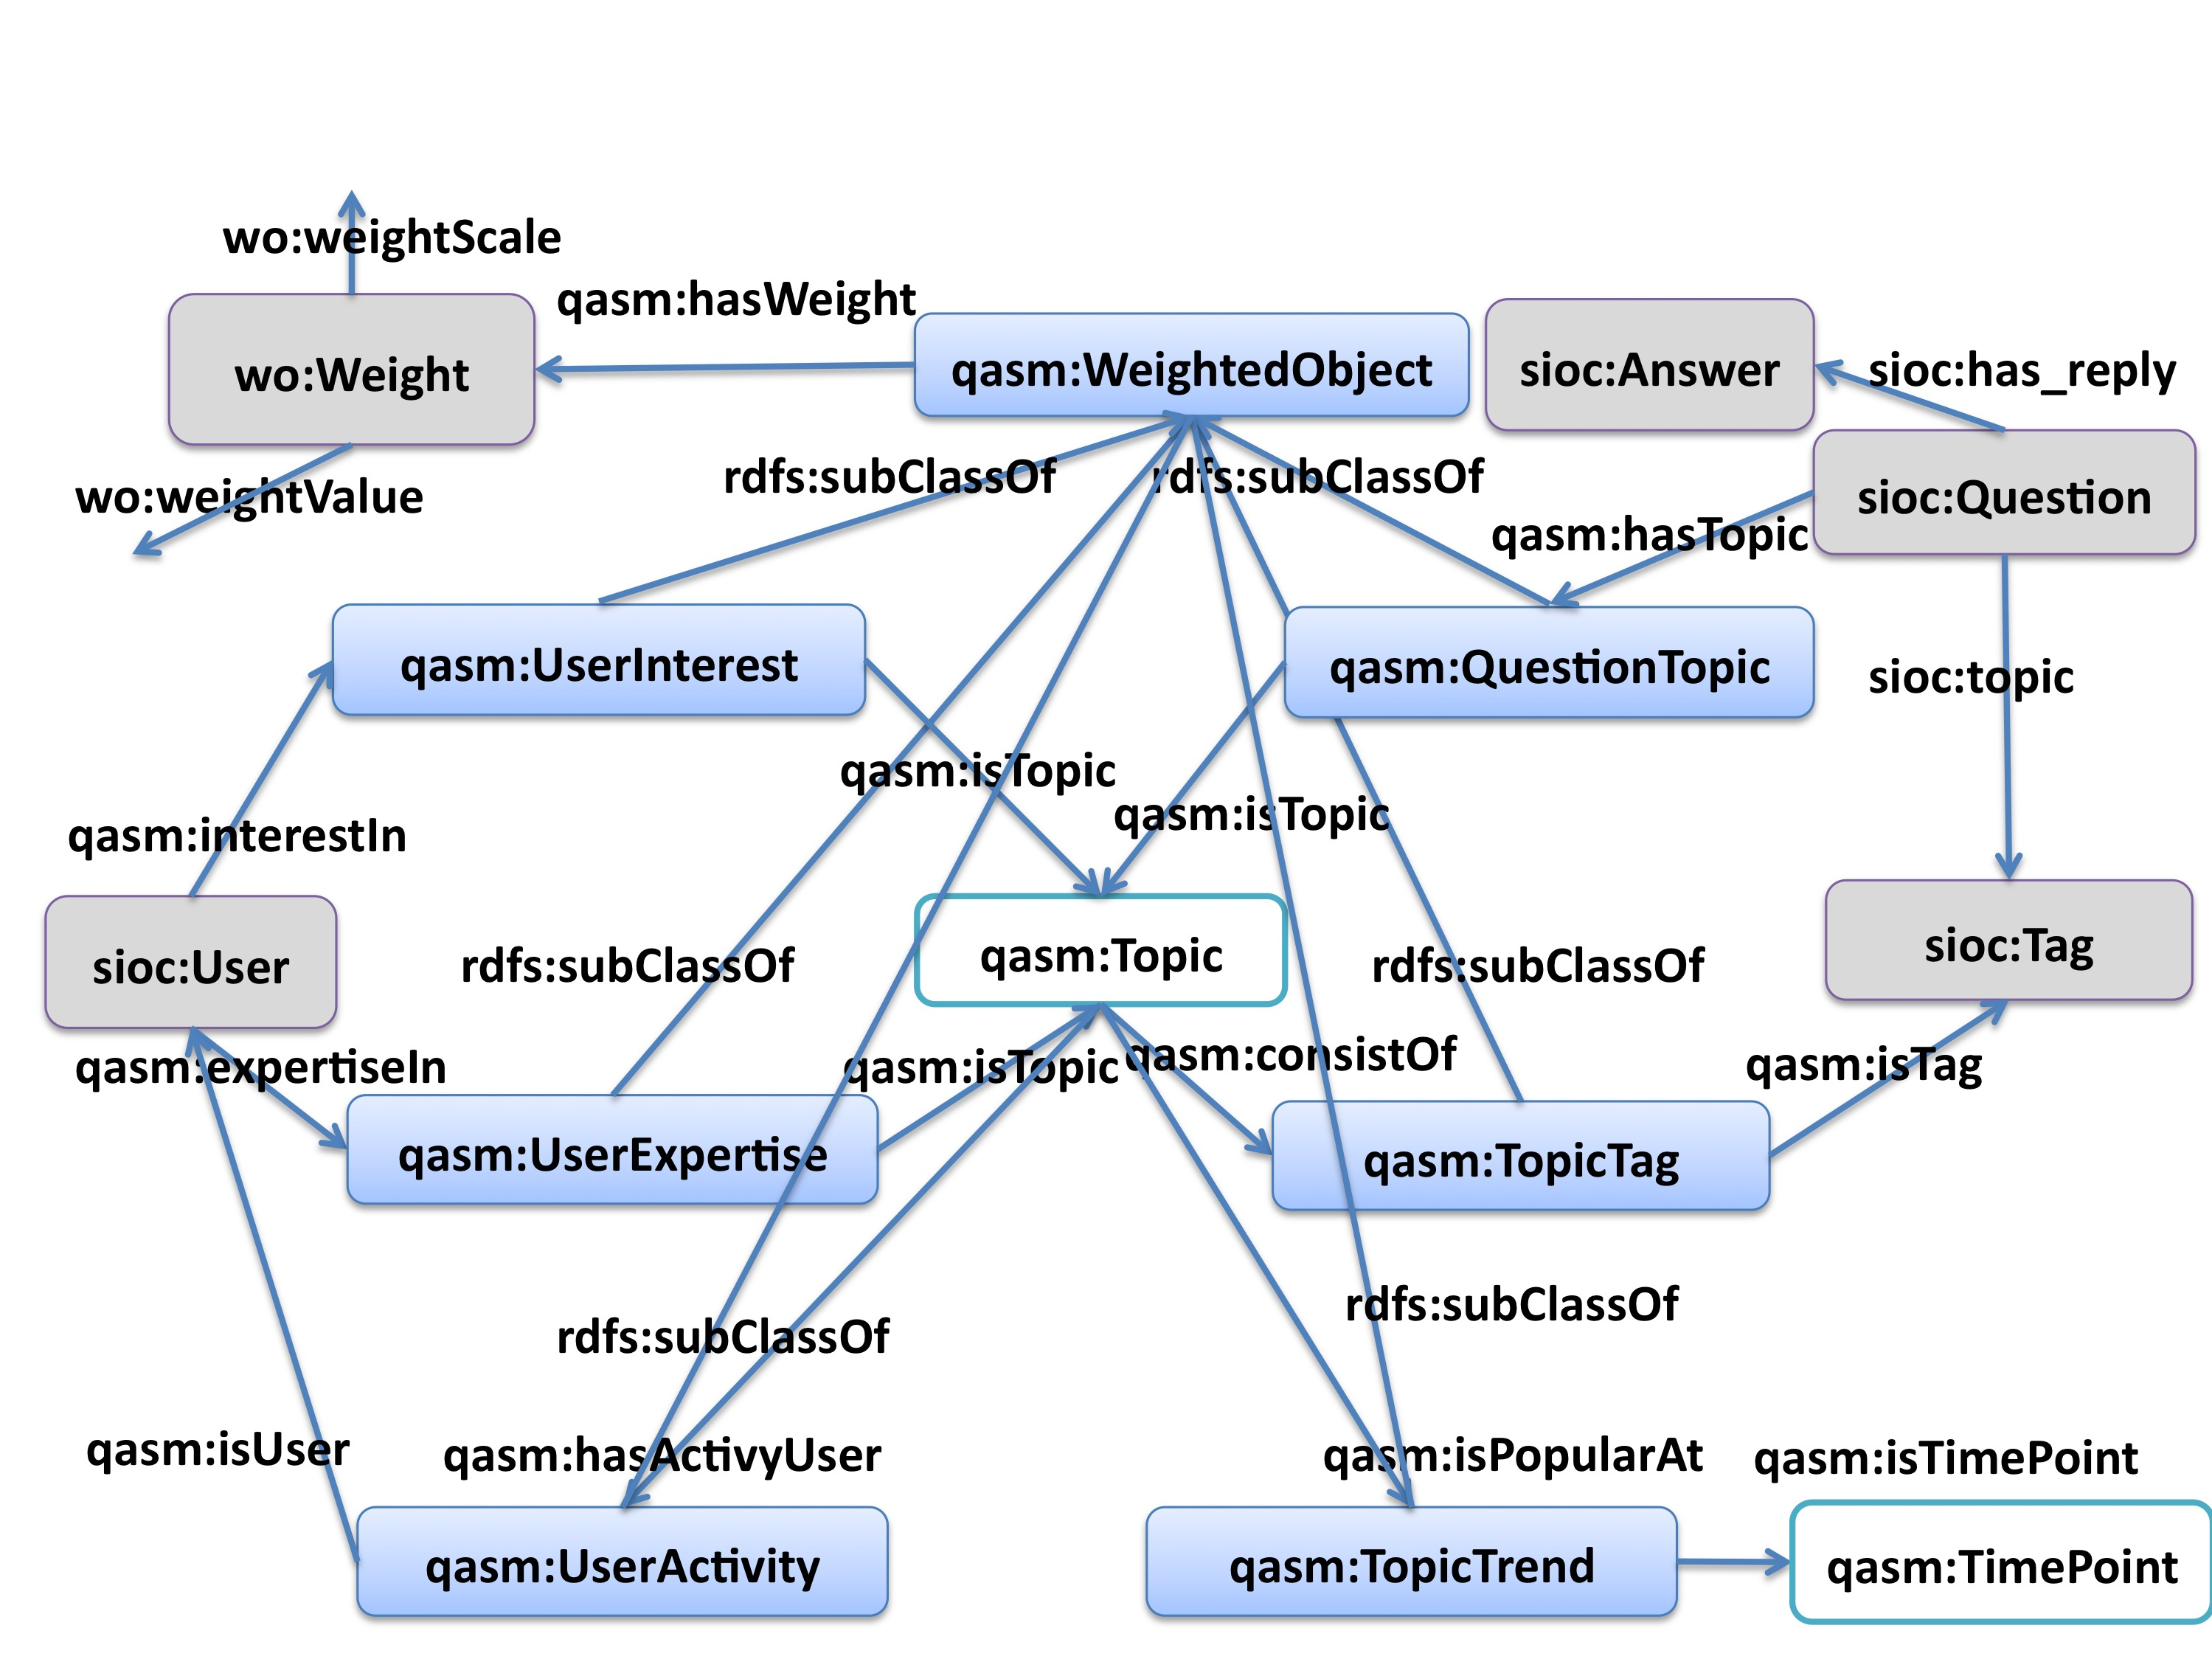
\includegraphics[width=8in]{qasm.jpg}
\caption{Overview of the QASM vocabulary}
\label{fig:coreontology} 
%\end{figure}
\end{sidewaysfigure}

As explained in the introduction, there are mainly two kinds of information to formalize. Part of it is explicit: the original user-generated content, such as Q\&A contents, user profile, votes, and timestamps. Part of it is implicit and extracted by social media mining techniques: user interests, overlapping communities, user expertise, user activities. 

Existing work mainly focus on how to formalize the explicit information in Q\&A sites. We are focusing on extending existing work to also formalize the implicit information. Thus, we proposed the QASM vocabulary\footnote{It is available online at \url{http://ns.inria.fr/qasm/qasm.html}}. Figure \ref{fig:coreontology} provides an overview of our ontology.
It reuses some class and property from SIOC (with soic: prefix), Dublin Core (with dcterms: prefix) and Weighted-Object (with wo: prefix)\footnote{\url{http://smiy.sourceforge.net/wo/spec/weightingontology.html} (accessed Aug 2016)}. 

% TODO: each and every notion above should be checked in LOV for alignment, reuse, comparison, etc.
%note zide checked and updated
%note zide try to reuse as much as possible. 
%note zide explained the added parts.
Table \ref{tab:qaontoclass} shows its main classes.
Table \ref{tab:qaontoproper} shows several properties used in our work. 

\begin{sidewaystable}
    \centering
    \begin{tabular}{|c|c|c|c|}
    \hline
    Class &  Description & Type & Ontology \\ \hline
    User  & active user & explicit &  sioc:User \\ \hline
    Question & questions post & explicit & sioc:Question \\ \hline
    Answer  & answer post & explicit & sioc:Answer \\ \hline
    Tag & tags used to label questions & explicit & sioc:Tag \\ \hline
    Word & words used in Q\&A content & explicit & qasm:Word \\ \hline
    PeriodOfTime & time interval & explicit & dcterms:PeriodOfTime \\ \hline
    Topic & bag of words/tags & implicit & sioc:Topic \\ \hline   
    UserInterest& User interest over topic distribution & implicit& qasm:UserInterest\\ \hline
    UserExpertise & User expertise over topic distribution &implicit& qasm:UserExpertise \\ \hline
    TopicTag &Topic over tags distribution&implicit &qasm:TopicTag \\ \hline
    
    TopicWord&Topic over words distribution &implicit & qasm:TopicWrod\\ \hline
    
    UserActivity&Topic over users distribution & implicit &qasm:UserActivity \\ \hline
    
    TopicTrend &Topic over time distribution &implicit & qasm:TopicTrend\\ \hline
          
    \end{tabular}
    \caption{the Vocabulary (classes) used in our work}
    \label{tab:qaontoclass}
\end{sidewaystable}


\begin{sidewaystable}
    \centering
    \begin{tabular}{|c|c|c|c|}
    \hline
        Property &  Description & Domain & Range  \\ 
    \hline
    qasm:interestIn  & links a user and a topic he is interested in & sioc:User &  qasm:UserInterest \\ \hline
    qasm:isTopic     & links a UserInterest declaration with a topic &qasm:UserInterest  &qasm:Topic \\ \hline
    qasm:hasWeight   & links a UserInterest declaration with a weight&qasm:UserInterest  &wo:Weight \\ \hline
    
    qasm:expertiseIn & links a user with as expertise & sioc:User & qasm:UserExpertise \\ \hline
    qasm:isTopic     & links a UserExpertise with a topic &qasm:UserExpertise &qasm:Topic \\ \hline
    qasm:hasWeight   & links a UserExpertise  with a weight &qasm:UserExpertise &wo:Weight \\ \hline
    
    qasm:consistOf   & links a topic with tags   &qasm:Topic &qasm:TopicTag \\ \hline
    qasm:isTag     & links a TopicTag with a tag  &qasm:TopicTag &sioc:Tag \\ \hline
    qasm:hasWeight   & links a TopicTag with a weight &qasm:TopicTag &wo:Weight \\ \hline
    
    qasm:consistOf   & links a topic with a TopicWord declaration  &qasm:Topic &sioc:TopicWord \\ \hline
    qasm:isWord     & links a TopicWord with a word  &qasm:TopicWord &sioc:Word \\ \hline
    qasm:hasWeight   & links a TopicWord with a weight &qasm:TopicTag &wo:Weight \\ \hline
    
    qasm:isPopularAt  & links a topic with a trend declaration & qasm:Topic &  qasm:TopicYearTrend \\ \hline
    qasm:isTimePeroid & links a TopicTrend with a time interval &qasm:TopicTrend  &dcterms:PeriodOfTime \\ \hline
    qasm:hasWeight   & alinks a TopicTrend with a weight&qasm:TopicTrend  &wo:Weight \\ \hline
    
    qasm:hasActiveUser & links a topic with an active user activity declaration & qasm:Topic &  qasm:UserActivity \\ \hline
    qasm:isUser     & links a user activity declaration with a user &qasm:UserActivity  &sioc:User \\ \hline
    qasm:hasWeight   & links a user activity declaration with a weight&qasm:UserActivity  &wo:Weight \\ \hline
          
    \end{tabular}
    \caption{the Vocabulary (properties) used in our work}
    \label{tab:qaontoproper}
\end{sidewaystable}

Since our work mainly generates distributions, we proposed a generic pattern to formalize these distributions. As an example, we show the formalization of a distribution in Figure \ref{fig:chp3ontoexample}. 

\begin{figure}%[htbp]
\centering
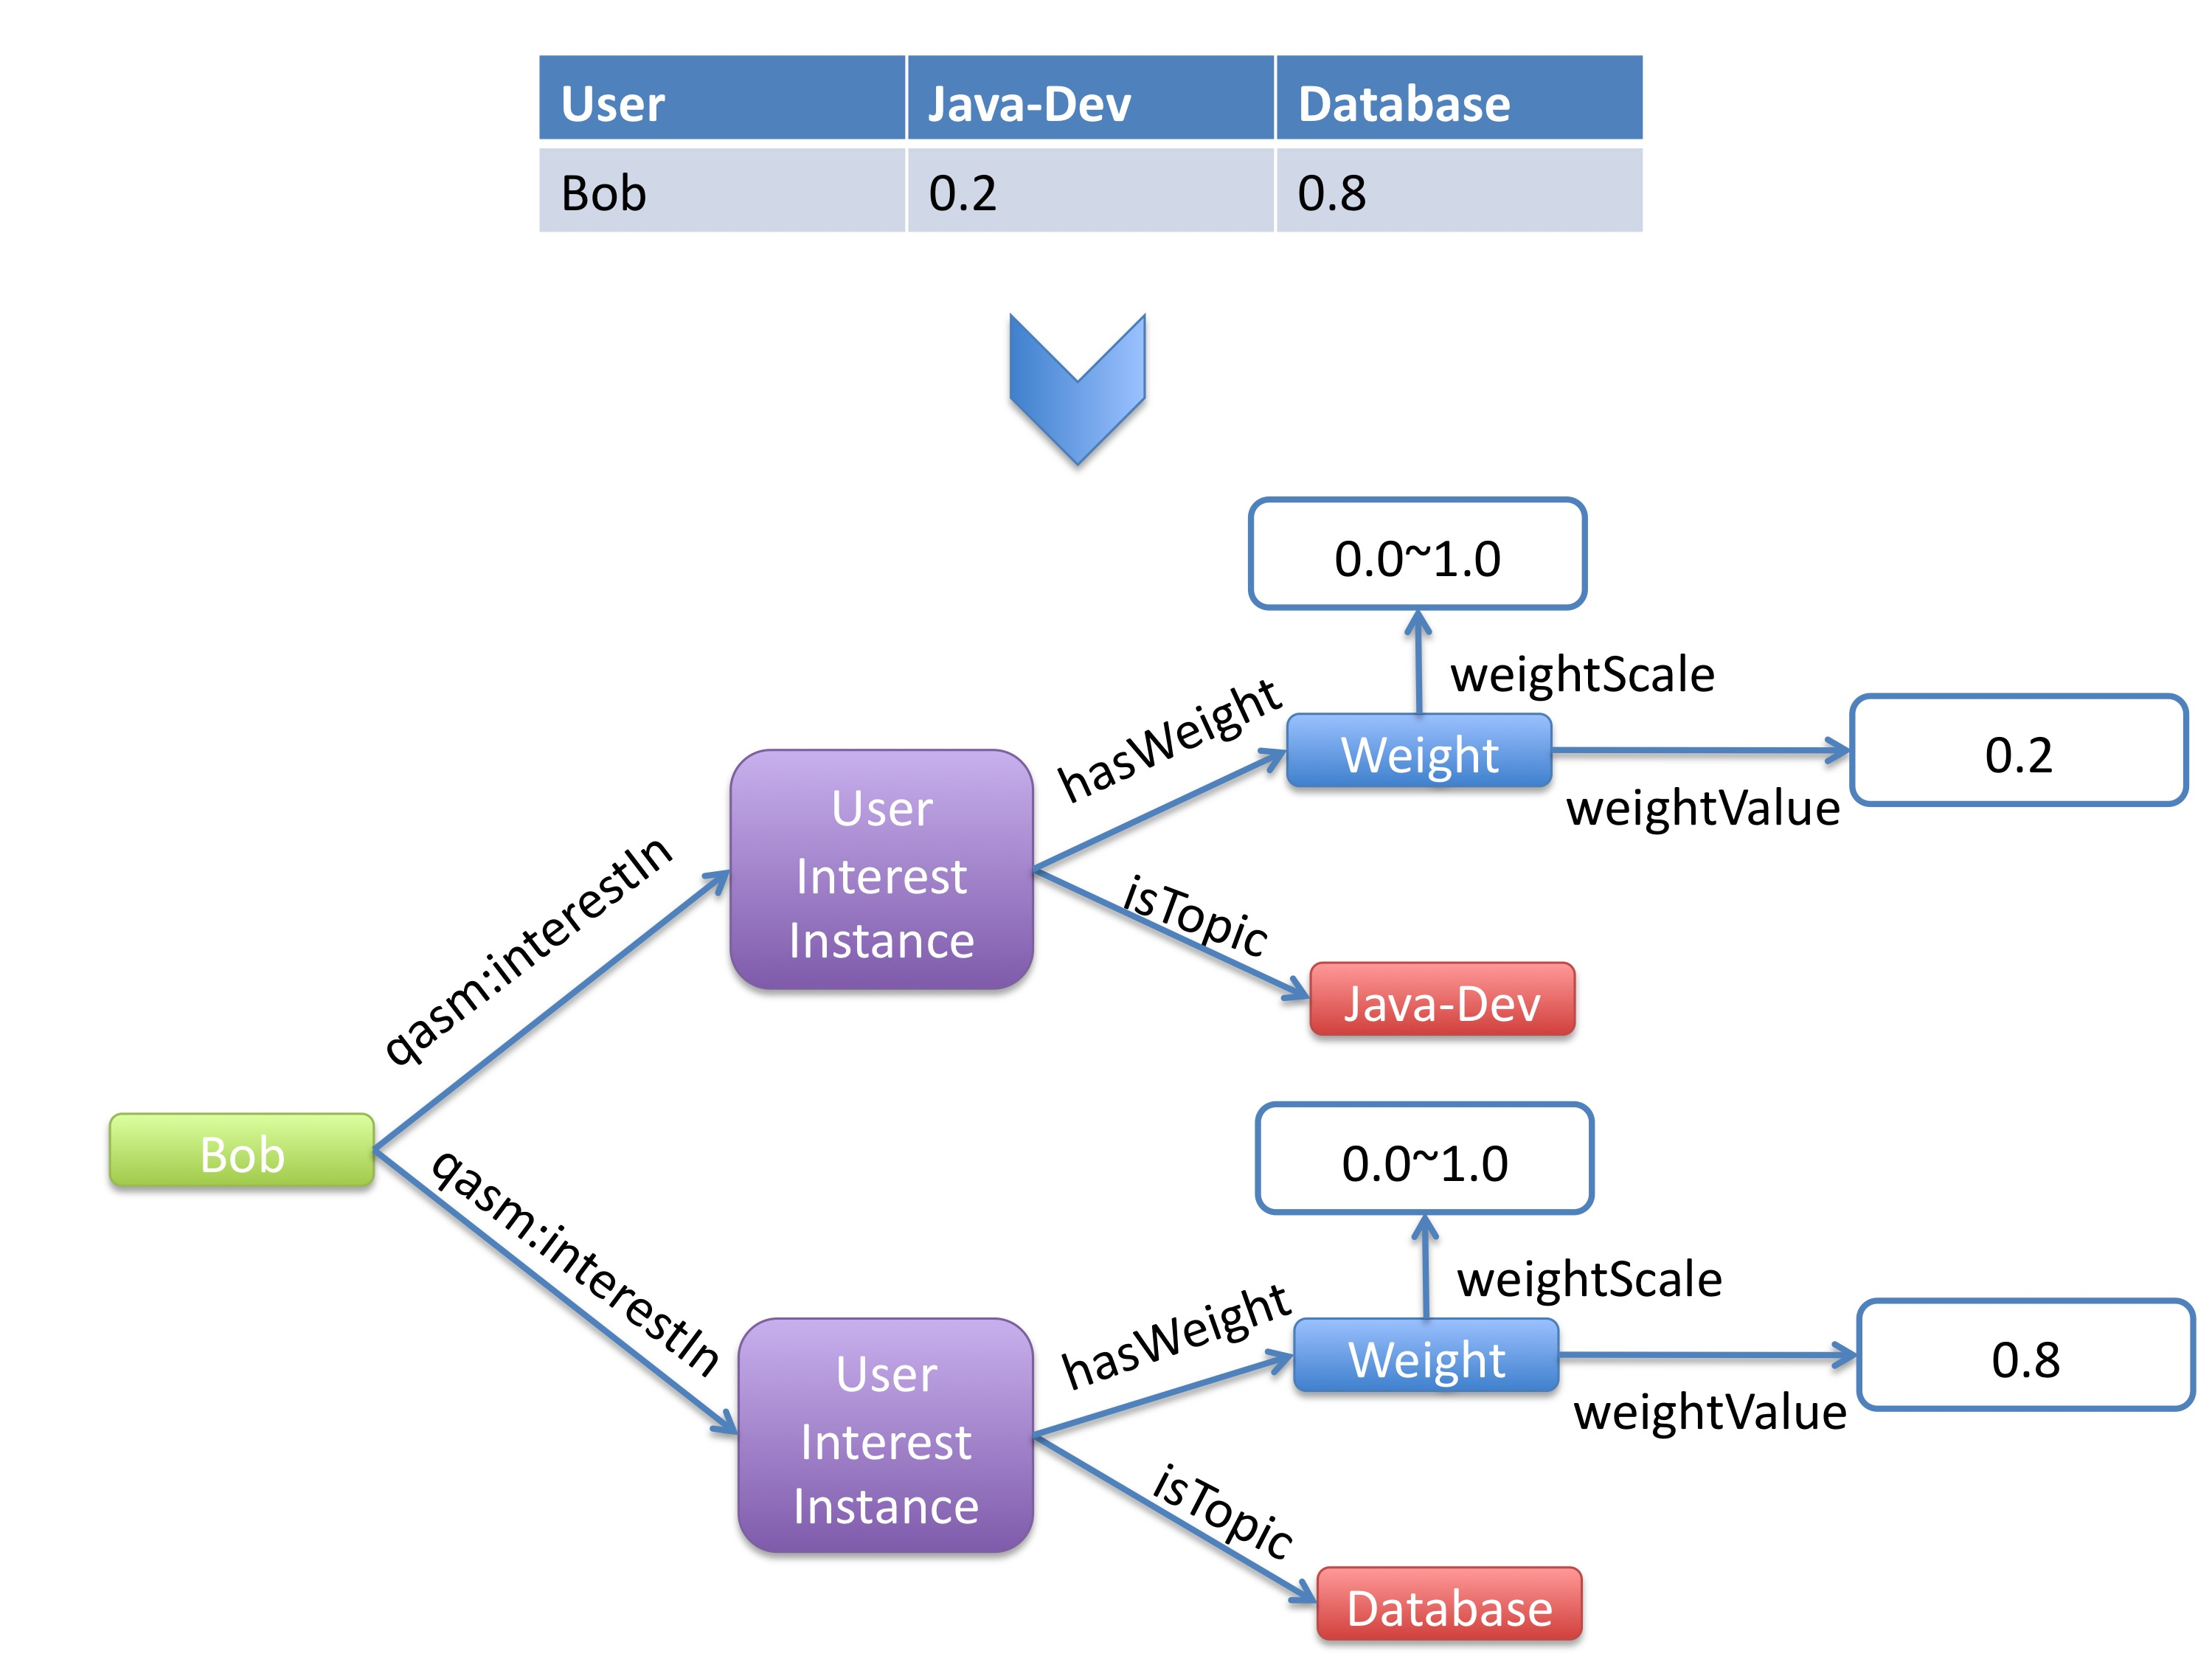
\includegraphics[width=5in]{chp3ontoExample.jpg}  
\caption{Example formalization of a distribution}
\label{fig:chp3ontoexample} 
\end{figure}

Here are the main new classes and properties introduced in the QASM vocabulary: 

\begin{itemize}
%\item \texttt{qasm:Topic}. SIOC, FOAF and Dublin Core  have Topic class. In FOAF, topic is defined as "a topic of some page or document",  We are different in a sense that in our definition, a topic is represented by a set of tags or a bag of word with weights. In our models, tags/words belong to instances of \texttt{qasm:Topic}, we also consider different tags/words have different weights/probablities/membership for each topic. 
%reuse sioc topic.

\item \texttt{qasm:WeightedObject} is used to describe the weight that a specified subject has with regard to a specified object. This class has four subclasses which represent question topics, users' interests, users' expertise and tag topics respectively. In fact, this class is used to model the distributions we extracted from the original data. For example, topic-tag distribution, user-interest distribution.
%not similar work

\item \texttt{qasm:interestIn} is used to describe the user-interest distribution. This property is different from \texttt{foaf:interest} for its range. In FOAF people are interested in documents, while in QASM a user is interested in a topic to a certain degree (a weight). In addition, our model of user interests to is quite similar to the WeightedInterest\footnote{\url{http://smiy.sourceforge.net/wi/spec/weightedinterests.html} (accessed Aug 2016)} ontology. The difference is that we mainly focus on formalizing the user-topic interest distribution on Q\&A sites. Besides, we also formalize expertise, trend, activity distribution on Q\&A sites.

\item \texttt{qasm:expertiseIn} is used to describe the user-expertise distribution. A user has different weights for different topics. The FRAPO ontology\footnote{\url{http://purl.org/cerif/frapo/hasExpertise} (accessed Aug 2016) } has a 'hasExpertise' property to describe a user having an expertise in a specified research area. Our model not only enables to describe a user having expertise on a topic, but also formalizes to what extent a user has expertise.

\item \texttt{qasm:isPopularAt} is used to describe the topic-time distribution. A topic has different popularity at different time interval.
%note zide did not found any similar.

\item \texttt{qasm:hasActiveUser} is used to describe the topic-user distribution. Different users perform different activities on a topic.
%note zide did not found any similar
\end{itemize}


% TODO: have you looked at the SCOT ontology? have you searched for your terms in the LOV directory ? example FOAF interest relation ? e.g. http://lov.okfn.org/dataset/lov/terms?q=interest
% This should be done for every primitive and the reasons for aligning or not should be given in the thesis. 

%note zide. checked.


\section{Formalizing Stackoverflow data with the QASM vocabulary}
%TODO you are missing one section describing the structure of the Stackoverflow data (dump), its format and the mapping between this structure and your vocabulary ; in other words in the introduction you say you will present the eaxtraction an formalization but you did not cover the extraction/mapping part. You need to add that to this chapter.
%done

We obtained the data dump of Stackoverflow from the website\footnote{\url{https://archive.org/details/stackexchange} (accessed Aug 2016)}. It includes all user-contributed content on the Stack Exchange network. Each site is formatted as a separate archive consisting of XML files. Each dataset includes Posts, Users, Votes, Comments, PostHistory and PostLinks and the schema information.

A first step is to map the original dataset to the QASM vocabulary. 
%Since the schema of the data dump are well organized and designed, we just simply mapped them one by one. 
%TODO Cath: this is not sufficient, you should briefly describe the structure of the data, and maybe provide an exemple and later on provide its translation in RDF/TUrtle using QASM

%We reuse as many as existing vocabularies: SIOC ontology (with prefix sioc: or tsioc:), Dublin Core (with prefix dcterm:), Reivew ontology (with prefix rev:), NEPOMUK Information Element Core Ontology (with prefix nie:). 
%TODO Cath you should not repeat again here which vocabularies are reused but the NIE ontology is not previously mentioned. You should do it in the section describing the QASM ontology
%For the "Posts.xml", 
%TODO Cath: what is Posts.xml
%note zide .the original dataset download from stackoverlfow.
The original schema elements and mapping QASM concepts are listed in table \ref{tab:mappingstackoverflow}.

\begin{sidewaystable}
    \centering
    \begin{tabular}{|c|c|}
    \hline
    Original Schema in Data dump & Mapping vocabulary in QASM \\ \hline
        Id       &  sioc:Id \\ \hline
        PostTypeId(1: Question, 2: Answer) & tsioc:Question, tsioc:Answer   \\ \hline
        ParentID (only present if PostTypeId is 2) & sioc:reply\_of   \\ \hline
        AcceptedAnswerId (only present if PostTypeId is 1) & qasm:acceptedAnswer  \\ \hline 
        CreationDate & dcterm:created \\ \hline
        Score & rev:totalVotes \\ \hline
        ViewCount & sioc:num\_views \\ \hline
        Body & nie:htmlContent\\ \hline
        OwnerUserId & sioc:has\_owner \\ \hline
        LastActivityDate & sioc:last\_activity\_date\\ \hline
        Title & dcterms:title\\ \hline
        Tags & sioc:Tag\\ \hline
        AnswerCount & sioc:num\_replies\\ \hline
        CommentCount & qasm:num\_comments\\ \hline
        FavoriteCount & qasm:num\_favorites\\ \hline
    \end{tabular}
    \caption{Mapping between original data dump of Stackoverflow and QASM vocabulary}
    \label{tab:mappingstackoverflow}
\end{sidewaystable}


\section{Modeling the latent knowledge in Q\&A sites}

Topics, interests, expertises, activities, trends are implicit  in the available raw CQA data. We use social media mining techniques to extract this knowledge.
In Chapter \ref{chap:ttd}, we propose a Tag Tree Distribution method to efficiently extract topics from tags. In Chapter \ref{chap:ttea}, we jointly model topic, interest, expertise and trend to extract the relations between them, such as user-topic, topic-time, user-expertise, user-interest etc. In Chapter \ref{chap:label} we propose a method using DBpedia to generate labels for the bags of words  used to define a topic and therefore to povide a label for the shared interests of a community. 
In the following we summarize the main notions that we will use in this thesis and give some examples of the latent knowledge extracted by our models. We also indicate the related vocabulary for each of them.

\begin{itemize}
\item \textbf{Topic}: A bag of words or tags which are closely related. Words are the content of questions or answers, tags are explicitly attached as such to questions. For example, the topic-tag distribution \textit{Database}:\{\textit{mysql}: 0.5, \textit{sql}: 0.3, \textit{query}: 0.2\}. expresses that topic \textit{Database} is related to tags \textit{mysql}, \textit{sql}, and \textit{query}. We use \texttt{qasm:TopicTag} and \texttt{qasm:TopicWord} to formalize this distribution.

\item \textbf{User Topical Interest}: A user is interested in different topics with different levels. For example, the user-topic distribution \textit{Alice}:\{\textit{Database}: 0.8, \textit{Java}: 0.2\} expresses that \textit{Alice} prefers to answer questions related to \textit{Database}, but rather not about \textit{Java}. We use \texttt{qasm:UserInterest} to formalize this distribution.

\item \textbf{User Topical Activity}:  Different users are interested in the same topic with different levels. For example, the topic-user distribution \textit{Database}:\{\textit{Alice}: 0.8, \textit{Bob}: 0.2\} expresses that \textit{Alice} prefers to answer questions related to \textit{Database}, while \textit{Bob} is not willing to contribute answers to it. We use \texttt{qasm:UserActivity} to formalize this distribution.

\item \textbf{Topic Trend}: A topic is popular at different points in time with different levels. For example, the topic-time distribution \textit{Database}:\{\textit{May/2013}: 0.2, \textit{June/2013}: 0.3, \textit{July/2013}: 0.5\} expresses that the topic \textit{Database} is increasingly popular. 
We use \texttt{qasm:TopicTrend} to formalize this distribution.

\item \textbf{User Topical Expertise}: A user has expertise in different topics with different levels. For example, the topic-expertise distribution for \textit{Alice} \textit{ios}:\{\textit{High}: 0.2, \textit{Medium}: 0.7, \textit{Low}: 0.1\} expresses that \textit{Alice}'s expertise on topic \textit{ios} is probably of medium level. We use \texttt{qasm:UserExpertise} to formalize this distribution.
\end{itemize}


\section{Summary: an effective way to manage Q\&A sites}
\label{sec:future}
We presented QASM, a Q\&A system and a vocabulary to combine social media mining and semantic Web models and technologies to manage Q\&A users and content in CQA sites. This chapter provided us with a general framework and vocabulary to capture user-generated content and extracted latent knowledge on Q\&A sites. In the next chapters, we will focus on how to efficiently extract this latent knowledge, such as topics and communities. And how to extract more latent information such as topic based temporal dynamics, topic based expertise.





